\section{Circuit Components and  New Language contructs}\label{sec:syntax}
We explored three reconfigurable circuit components and designed three kinds of new language constructs accordingly to describe them. The syntaxes are $fold$, $map$ and $forloop$ which portray the computation meanings of the reconfigurable structures.

\subsection{Fold}
The fold is something like higher order function\cite{highorderfunction} "$fold$" (or "$reduce$") in Haskell. Typically, we can use $fold$ to model a circuit that calculates the following mathmatical expression:
%\vspace{-3ex}
\begin{equation} \label{eq:fold} sum = (var << s_n) + ... + (var << s_0) \end{equation}
It shifts $var$ by $s_n$,...,$s_0$ and then sums up the shifting results, stores the final value in register $sum$.
%\vspace{-2ex}
%%%%%%%%%%%%%%%%%%%%%%%%%%%%%%%%%%%%%%%%%%%%%%%%%%%%%%%%%%%%%%%%%%%%%%%%%%%%%%%%%%
%\begin{figure}
%  \centering
%  \begin{minipage}[thbp]{0.4\linewidth}
%     \centering
%     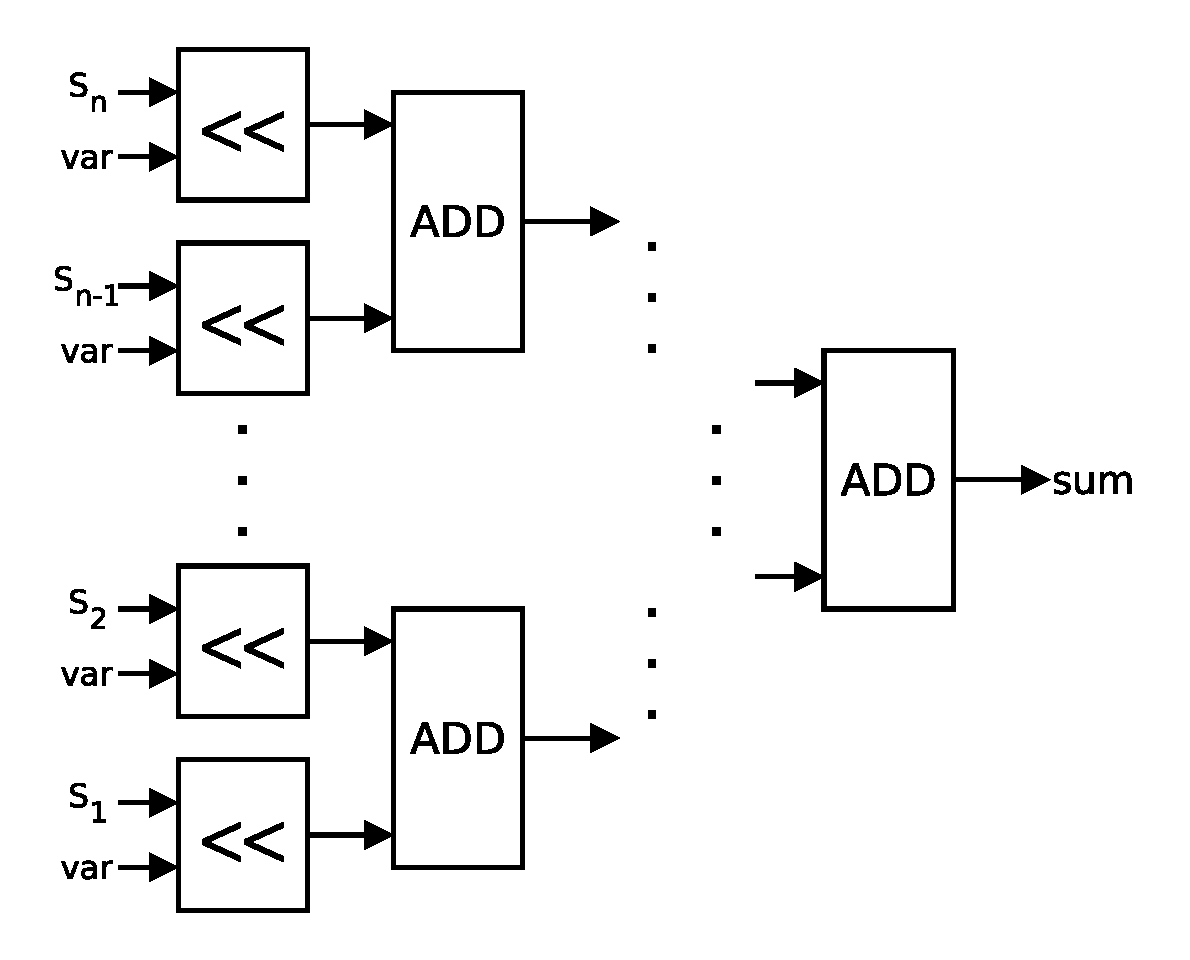
\includegraphics[width=\columnwidth]{fold}
%  \end{minipage}
%  \begin{minipage}[thbp]{0.4\linewidth}
%     \centering
%     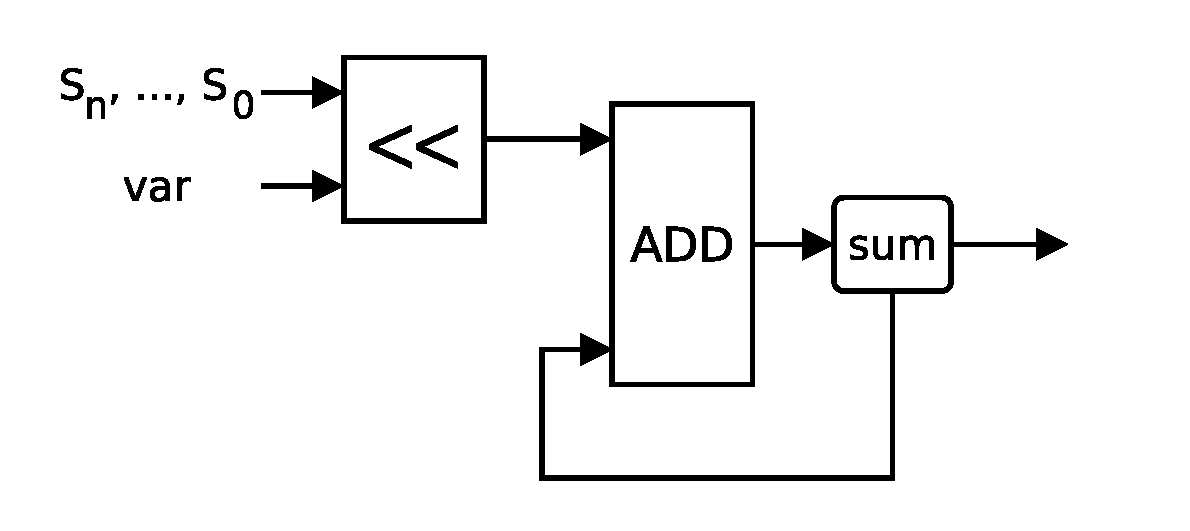
\includegraphics[width=\columnwidth]{fold3}
%  \end{minipage}
%  \caption{Different Circuit Architectures for Eq\eqref{eq:fold}}
%  \label{fig-fold}
%\end{figure}
%%%%%%%%%%%%%%%%%%%%%%%%%%%%%%%%%%%%%%%%%%%%%%%%%%%%%%%%%%%%%%%%%%%%%%%%%%%%%%%%%%
\begin{figure}[ht]
\centering
\subfigure[]{
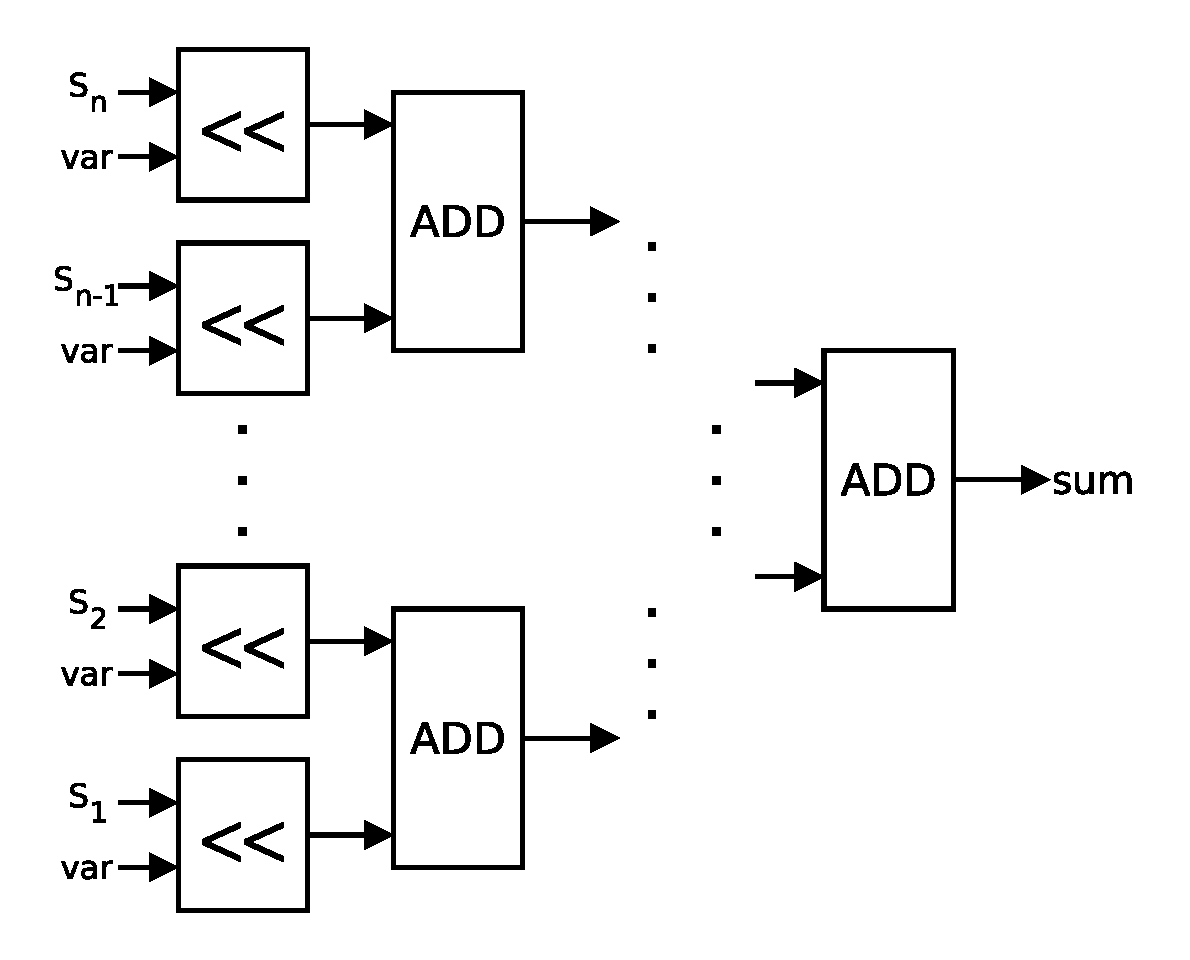
\epsfig{file=fold.eps, width=0.4\columnwidth}
%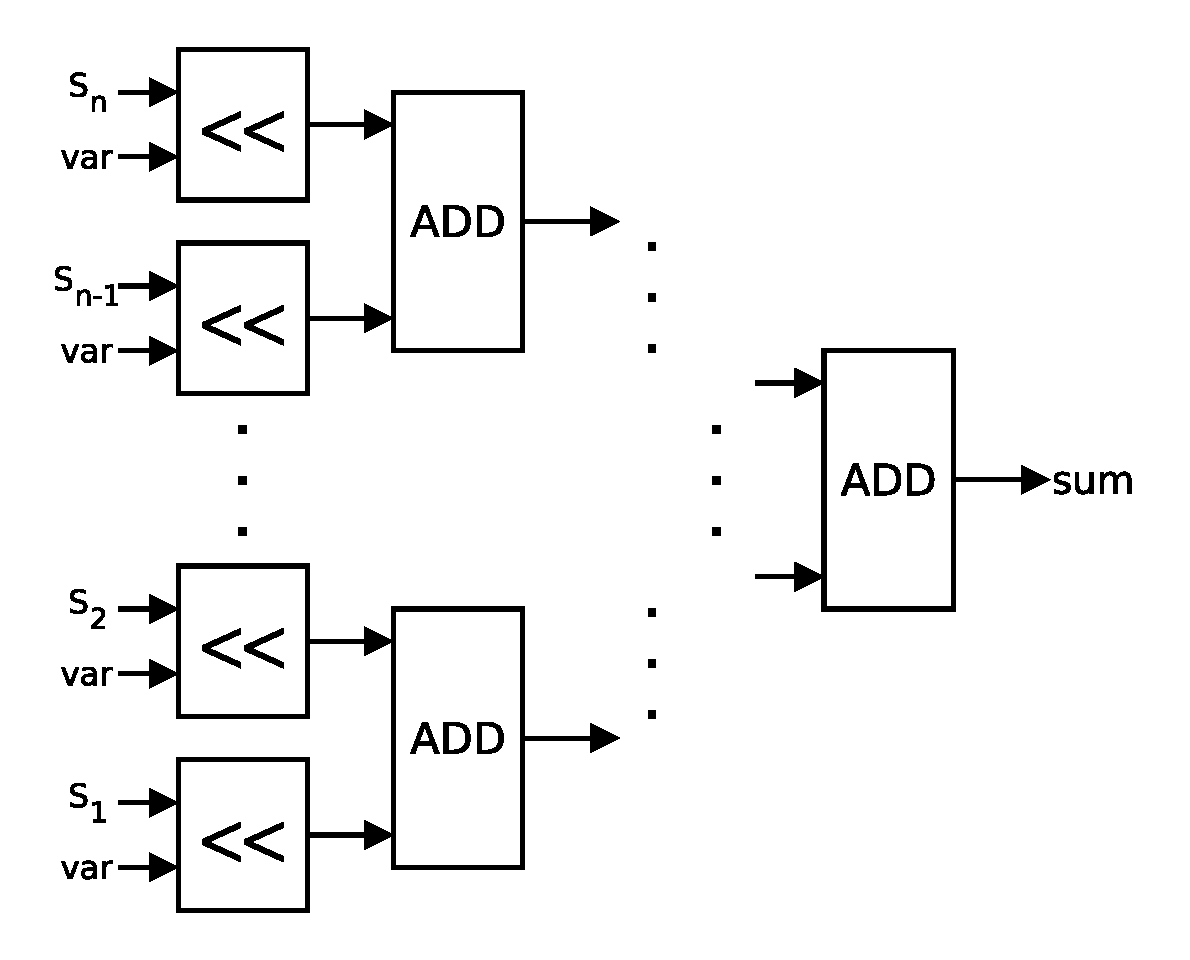
\includegraphics[scale=0.3]{fold}
}
\subfigure[]{
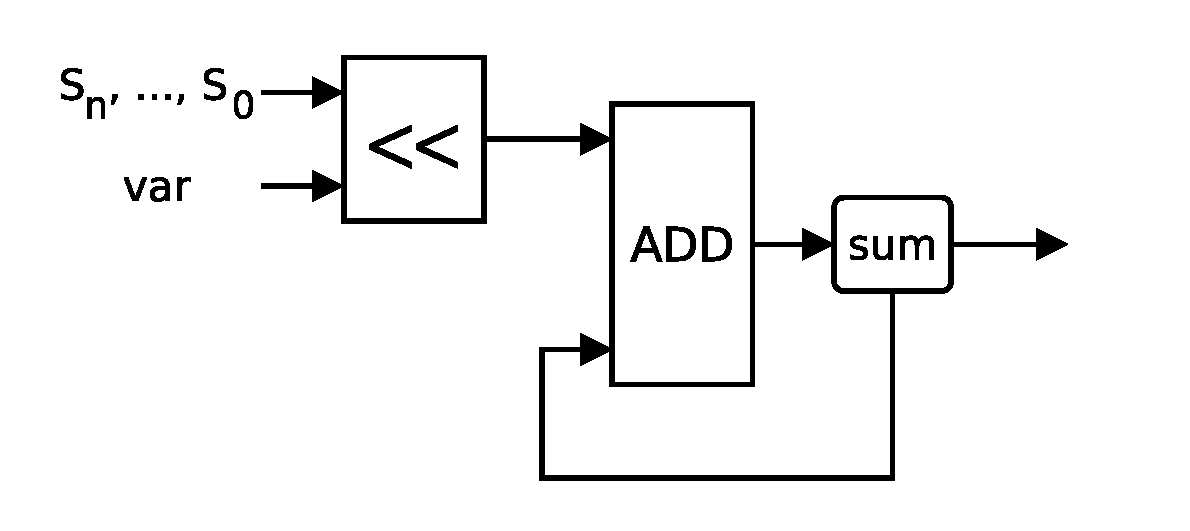
\epsfig{file=fold3.eps, width=0.4\columnwidth}
%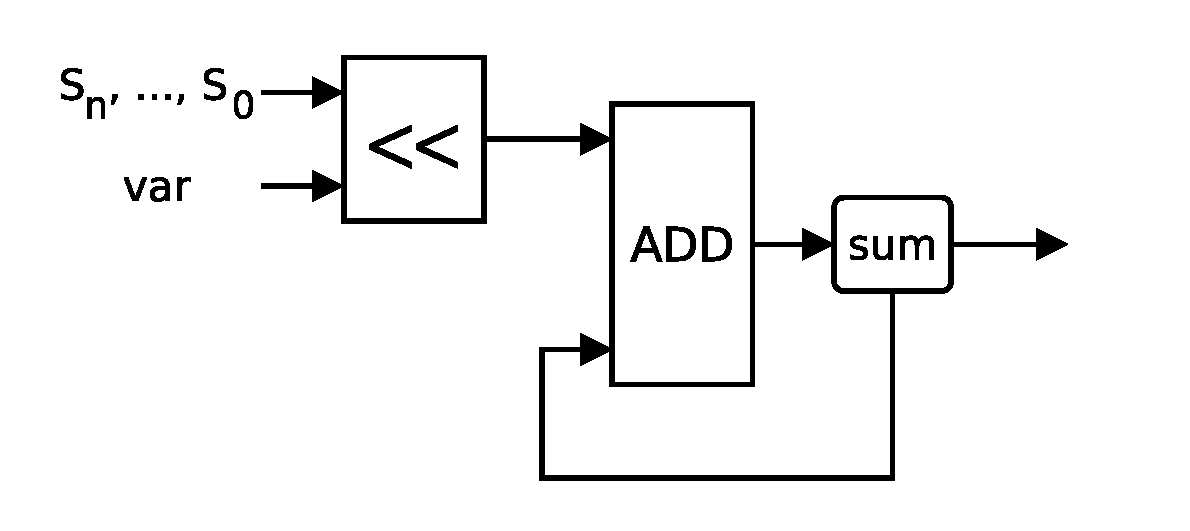
\includegraphics[scale=0.3]{fold3}
}
%\vspace{-2ex}
\caption{Different Circuit Architectures for Eq\eqref{eq:fold}}
\label{fig-fold}
\end{figure}
%\vspace{-2ex}
Fig \ref{fig-fold} gives two distinct implementations of expression \eqref{eq:fold}. We should be aware of that these are only two among dozens of architectures that can describe the dataflow of implementations of equation \eqref{eq:fold}. Question here is HDL languages, such as Verilog, just can describe only one implementation's architecture in one copy of code. For different architectures,designer needs to write different copies of source code in HDL. However, we can generalize these implementations by highlighting the re-configurable part, using the following syntax.

\begin{verbatim}
         fold(sum,var,sn,. . .,s0)
\end{verbatim}
where, $sum$ and  $var$ hold input $x$ and output $y$, $sn,...s0$ are the input variables which indicate the shift length.
\\
This "fold" syntax hides the architecture details of implementation of formular \eqref{eq:fold}, we can just use it to express a range of different implementations.
\subsection{Map}
$Map$ is used to model the circuit that does some operations upon a list of data. It's also similar to higher order function "$map$" in Haskell. In Haskell, $map$ takes two inputs - a function, and a list. It then applies this function to every element in the list. In Verilog we don't have list type. However we can view a $reg$ or $wire$ as a bit list, and every time we applies the function (actually we should call it a $module$ in circuit design) to a slice of the bits. Figure \ref{fig-map} shows the $map$ structure, as an example, we can think  "Module" has the functionality that adds 1 to the input data list. Here comes the syntax of $map$:

\begin{verbatim}
         map(md,data,datalen,maplen)
\end{verbatim}
where $md$ is a module identifier, $data$ is the bit-list name (variable name of a $reg$ or $wire$), $datalen$ is the length of the bit-list and $maplen$ is the length of the bit slice that applied to the module each time.
%\vspace{-2ex}
\begin{figure}[ht]
\centering
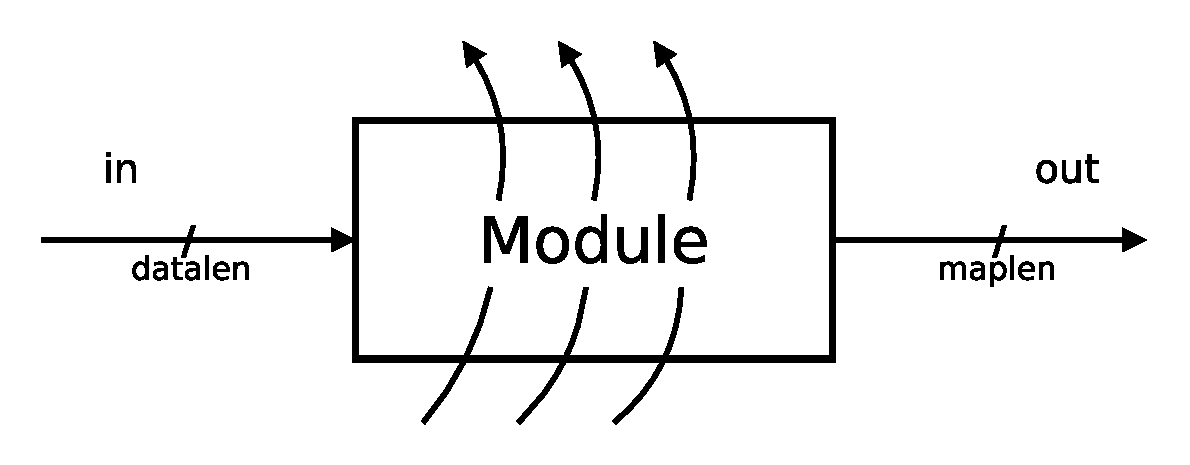
\epsfig{file=map.eps,width=0.5\columnwidth}
%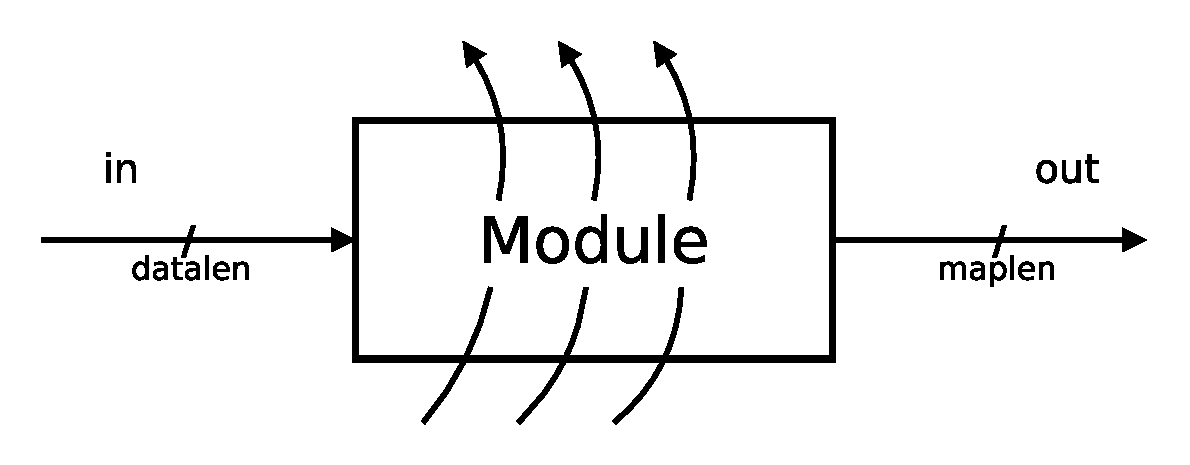
\includegraphics[scale=.5]{map}
%\vspace{-2ex}
\caption{Map Circuit Structure}
\label{fig-map}
\end{figure}

\subsection{Forloop}
As we know, operation got executed repeatedly in a $forloop$.
One of the most important features of High Level Synthesis\cite{Tutorial:HLS} for tuning design performance is Loop Unrolling\cite{Verilog:Loop}. Here is a simple forloop example in C/C++:
%\vspace{2ex}
%\hrule
%\vspace{-3ex}
\begin{verbatim}
for(i=0;i< 4;i++)
   sum += a[i];
\end{verbatim}

Traditionally, in some low level optimizations, the $forloop$ got unrolled or partial unrolled:
%\vspace{2ex}
%\hrule
%\vspace{-3ex}
\begin{verbatim}
FULLY UNROLL:     |   PARTIAL UNROLL:
  sum += a[0];    |   for(i=0; i<4; i+=2)
  sum += a[1];    |      sum += a[i];
  sum += a[2];    |      sum += a[i+1];
  sum += a[3];    |
\end{verbatim}

Obviously, different unrolling strategies result in diverse circuits.
However, a copy of HDL code just implements one optimization, multiple copies of code are necessary to provide all possible optimized IP core. In SV+,a new syntax for expressing a $forloop$ is proposed:(take the C/C++ $forloop$ as a demo)
%\vspace{2ex}
%\hrule
%\vspace{-3ex}   
\begin{verbatim}
always@(posedge clk)
if(for_i)
for
   sum += a[0];
   sum += a[1];
   sum += a[2];
   sum += a[3];
end
\end{verbatim}
Where, $clk$ and $for\_i$ are control signals that triage the execution of this loop. So firstly, this loop can be synthesized into a sequential block. Secondly, further optimization choices (mainly the depth of unrolling) are provided by the compiler. The programmer, especially someone who has little circuit design experience, has the chance to choose an optimization option via interacting with the compiler.     
